\documentclass[french]{llncs}

\usepackage[english, french]{babel}
\usepackage[utf8]{inputenc}


\usepackage{graphicx}
\usepackage{float}
\usepackage{booktabs}
\usepackage{amsmath}
\usepackage{listings}
\usepackage{subfig}
\usepackage{hyperref}

%-----------------------------------------
\title{ Comparaison de modèles GNN pour la prédiction de liens }

%\subtitle{\vspace{.5cm}Rapport de Master}

\author{ Yann  \textsc{Amer} \\
         Jules \textsc{Cairole} \\
         Nicolas \textsc{Dapzol} 
          }
\institute{Université Claude Bernard Lyon 1, France}

\lstset{ 
    basicstyle=\small,
    captionpos=b  % sets the caption-position to bottom
}
\setlength{\intextsep}{6pt}
\setlength{\textfloatsep}{6pt}
\setlength{\floatsep}{6pt}




\providecommand{\motcles}[1]{\textbf{Mots-clés:} #1}

\pagestyle{headings} 
%-----------------------------------------

\begin{document}

    \renewcommand{\thelstlisting}{\arabic{lstlisting}}

    \maketitle   
    
    \selectlanguage{english}
    \begin{abstract}
        This study aims to compare different parameterization of a VGAE to predict links.
        We use airport database to make the experiment. We show that a simple model with chosen paraemeters outperforms more complex one.
        
         \begin{keywords}
        GNN, VGAE, SAGE
    \end{keywords}
    \end{abstract}


   

%-----------------------------------------

    \section{Introduction  } \label{intro}

L'étude vise à comparer plusieurs modèles VGAE dans le cas particulier de la prédiction de liens entre aéroports.  Il a pour objectif de présenter et de valider l'utilisation d'un modèle pour un tel objectif et sélectionner une première approche.  L'ensemble des résultats est reproductible en suivant ce dépôt \href{https://github.com/nicolasdapzol/projetGNN_airport.git}{ lien GITHUB}.
        
       % Toutes les instructions détaillées concernant l'utilisation de la classe \textit{llncs.cls}, ainsi que les templates \LaTeX. et \texttt{Word}, sont téléchargeables sur la page suivante:\\ \url{https://www.springer.com/gp/computer-science/lncs/conference-proceedings-guidelines}.\\
        
    % Le rapport de projet doit faire maximum 4 pages (hors refs). Vous pouvez l'écrire en Français ou en Anglais mais l'abstract doit être en Anglais.
      
      
 \section{Etat de l'art : } 
Les Graph Neural Networks sont des architectures conçues pour traiter des données structurées sous forme de graph et permettre un apprentissage des caractéristiques du réseau. 
Les graph auto encoders sont une famille particulière. Elles visent à synthétiser les données puis à les reconstruire. Ceci permet de voir émerger des structures internes aux données. Les Variational Graph Auto-encoders \cite{article} en sont une extension. Ces modèles modélisent l'espace latent par un espace probabiliste où chaque noeud est représenté par une gaussienne (avec pour paramètres sa moyenne et sa variance).
Ce type de graph a pour avantage son interprétabilité, sa robustesse et ses capacités généralisatrices \cite{yang2024variationalgraphautoencoderbased}. 
Différents noyaux peuvent être mobilisés : 
\begin{itemize}
    \item Graph Convolutional Network (GCN) Kipf \& Welling, 2017 \cite{DBLP:journals/corr/KipfW16}. 
    \item Graph Attention Network (GAE) \cite{kipf2016variationalgraphautoencoders}
    \item Graph Sample and Aggregation (GraphSAGE) \cite{DBLP:journals/corr/HamiltonYL17}
\end{itemize}
Les spécifications sont nombreuses pour leurs implémentations, nous proposons dans ce papier d'étudier l'effet des différents noyaux et de plusieurs hyperparamètres pour une étude de cas spécifique. 

 \section{Présentation et transformation des données :  }
 
Le graphe représente le réseau aérien mondial : chaque nœud est un aéroport et chaque lien une route directe, non orientée. Il compte 3\,363 aéroports, répartis dans 212 pays, et 13\,547 routes. Le nombre de routes par aéroport (le degré) est très hétérogène : la médiane vaut 3, la moyenne 8,1 et le maximum 248, ce qui traduit la présence de quelques aéroports très connectés. Le graphe est quasi connexe : sur ses 6 composantes connexes, une composante géante regroupe 3\,351 aéroports (99,6\,\%), les 5 autres étant de petits îlots de 2 à 4 aéroports. Enfin, le coefficient de clustering moyen de 0,49 indique qu'environ la moitié des couples de voisins d'un aéroport sont eux-mêmes reliés.

\begin{figure}[H]
\centering
\begin{minipage}[c]{0.38\linewidth}
  \centering
  \small
  \begin{tabular}{lr}
    \toprule
    Indicateur & Valeur \\
    \midrule
    Aéroports (nodes) & 3\,363 \\
    Routes (edges) & 13\,547 \\
    Degré moyen & 8,1 \\
    Degré médian & 3 \\
    Degré max & 248 \\
    Composantes connexes & 6 \\
    Clustering moyen & 0,49 \\
    Nombre de pays & 212 \\
    \bottomrule
  \end{tabular}
  \captionof{table}{\small Caractéristiques du graphe.}
\end{minipage}\hfill
\begin{minipage}[c]{0.58\linewidth}
  \centering
  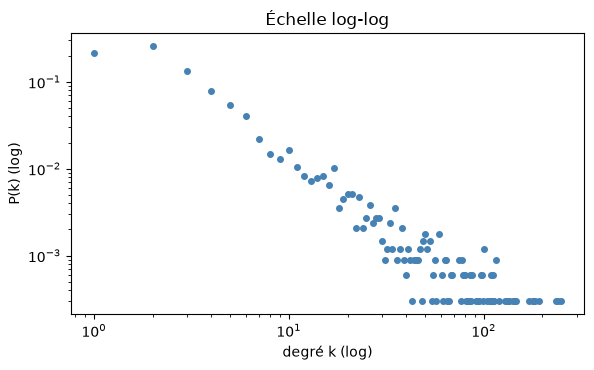
\includegraphics[width=\linewidth]{log-log.png}
  \captionof{figure}{\small Distribution des degrés (échelle log-log) : la plupart des aéroports ont peu de routes, quelques hubs en ont plus de 200.}
\end{minipage}
\end{figure}

Chaque aéroport est décrit par quatre caractéristiques : longitude, latitude, population et pays. Nous comparons trois jeux de features : (1) longitude, latitude et population normalisées (3 dimensions) ; (2) les coordonnées sur la sphère, avec la latitude et la longitude, plus $\log(1+\text{population})$ standardisée (4 dimensions) ; (3) le jeu (2) complété par le pays encodé en one-hot (216 dimensions).

\begin{figure}[H]
\centering
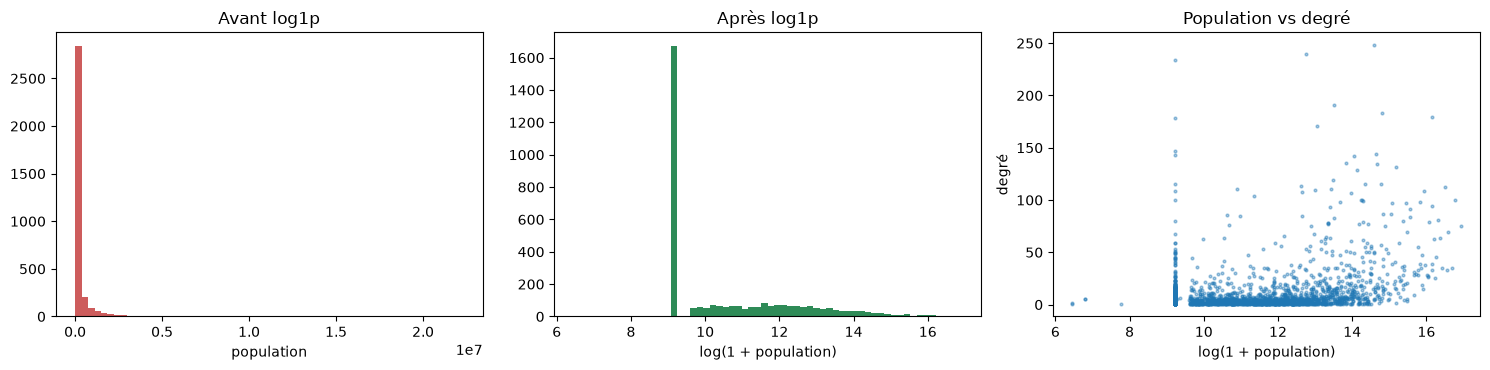
\includegraphics[width=\linewidth]{log(1+p).png}
\caption{\small Population avant et après $\log(1+x)$, puis lien avec le degré : la transformation corrige l'asymétrie, et le pic à 10\,000 correspond à une valeur par défaut (environ 50\,\% des aéroports).}
\end{figure}

\paragraph{Nécessité de l'encodage one-hot.}
Le pays est une variable catégorielle : un GNN ne peut pas exploiter du texte. Le coder par un entier (0 à 211) imposerait un ordre et des distances artificielles entre pays. L'encodage one-hot associe à chaque pays un vecteur de 212 composantes avec un seul 1, ce qui rend tous les pays équidistants. A noter que 57,4\,\% des vraies routes relient deux aéroports du même pays, contre 5,4\,\% pour des paires tirées au hasard.

  
 
 \section{Modèles et résultats:   }

 Les données sont réparties en 3 sous-ensembles app(80\%),val 10\%, test 10 \%. Pour chaque modèle, 3 essais sont effectués avec des valeurs d'initialisation différente.

\textbf{Sélection du noyau  : }
Dans un premier temps, trois types de convolution ont été testés: GCN, GAT, SAGE. Celui avec les meilleures valeurs moyennes d'AUC et d'AP pour la validation étant le GCN, c'est celui-ci qui est conservé pour la suite.\ref{tab_compar}\\
\textbf{Sélection du nombre de neurones  : }
Par la suite, le nombre de neurone a été testé. GCN\_128 obtient de meilleures performances que GCN\_32 (écart supérieur à la variabilité entre seeds). GCN\_128 a été retenu, malgré 4 fois plus de paramètres, pour un temps d'entraînement équivalent.\\
\textbf{Sélection des hyperparamètres: }
Enfin, la valeur de learning rate a été optimisée. Les learning rates 0.005 et 0.01 donnent des performances équivalentes (écart inférieur à la variabilité entre seeds). Nous retenons GCN\_128\_1 : avec early stopping, il converge en environ 120 epochs contre 180 (temps divisé par 1.5).
\\
\textbf{Modèle final avant ablation }
Les valeurs pour le modèle retenu GCN(128$\rightarrow$ 16) et  lr = 0.01, sur le test\_data sont les suivantes : \\
AUC test =  0.9729 $\pm$ 0.0012\\
AP test =  0.9754 $\pm$ 0.0016



{
\renewcommand{\arraystretch}{1.25}
\small
\begin{table}[H]
\centering
\caption{Comparaison des différentes implémentations (moyenne ± écart-type sur 3 seeds).}
\label{tab_compar}
\begin{tabular}{l c c c c c c c c}
\toprule
\textbf{Modèle} & \textbf{Noyau} & \textbf{Hidden} & \textbf{Out} &
\textbf{LR} & \textbf{Epoch} &
\textbf{AUC val} & \textbf{AP val} & \textbf{Temps} \\
\midrule
GCN\_32 & GCN & 32 & 16 & 0.01 & 164 &
0.9751±0.0011 & 0.9761±\textbf{0.0002} & 1.39 \\
GAT & GAT & 32 & 16 & 0.01 & 173 &
0.9293±0.0059 & 0.9203±0.0111 & 2.06 \\
SAGE & SAGE & 32 & 16 & 0.01 & 141 &
0.9263±0.0041 & 0.9282±0.0107 & 1.40 \\
\midrule
\textbf{GCN\_128\_1} & GCN & 128 & 16 & 0.01 & 123 &
\textbf{0.9775}±0.0017 & \textbf{0.9785}±0.0017 & 1.43 \\
GCN\_6 & GCN & 6 & 6 & 0.01 & 293 &
0.9606±0.0049 & 0.9630±0.0031 & 1.61 \\
GCN\_128\_2 & GCN & 128 & 16 & 0.005 & 182 &
0.9773±0.0014 & 0.9783±0.0019 & 2.14 \\
GCN\_128\_3 & GCN & 128 & 16 & 0.05 & 90 &
0.9697±\textbf{0.0007} & 0.9704±0.0016 & \textbf{1.00} \\
\bottomrule
\end{tabular}
\end{table}
}



 \section{Ablation Study }
 \textbf{Ablation de l'architecture : }
Retirer la partie variationnelle (GAE) réduit légèrement les performances en validation (AUC $-0.0024$). Le terme KL agit surtout comme une régularisation : il retarde le surapprentissage (minimum de la loss de validation vers l'epoch 120, contre 60 pour le GAE). Retirer la couche cachée (VGAE 1 couche) augmente légèrement les performances (AUC val $-0.0012$, de l'ordre de la variabilité entre seeds), avec 4 fois moins de paramètres et des résultats plus stables. La couche cachée n'est donc pas indispensable ; elle permet seulement une convergence deux fois plus rapide (123 epochs contre 251).\\
\textbf{Ablation des données : }
La normalisation est la transformation la plus importante : sur les features brutes, le modèle n'apprend presque pas (AUC $\approx 0.65$), la population écrasant les coordonnées. Les coordonnées 3D améliorent ensuite nettement les performances (AUC val $+0.0052$ par rapport aux features normalisées). En revanche, l'ajout des pays en one-hot (216 features) n'apporte pas de gain : data\_2 (4 features) est équivalent en validation et meilleur sur le test (AUC $0.9762$ contre $0.9729$), l'information sur le pays étant en grande partie redondante avec la position géographique.\ref{tab_ablation}
{
\renewcommand{\arraystretch}{1.25}
\small
\begin{table}[H]
\centering
\caption{Ablation study : impact des composants du modèle et des données (sans métriques test).}
\label{tab_ablation}
\begin{tabular}{l l c c c c}
\toprule
\textbf{Ablation} & \textbf{Retrait} & \textbf{Epoch} &
\textbf{AUC val} & \textbf{AP val} & \textbf{Temps} \\
\midrule
\multicolumn{6}{c}{\textit{Ablation de l'architecture (data\_3)}} \\
\midrule
VGAE (final) & -- & 123 & 0.9775±0.0017 & \textbf{0.9785}±0.0017 & 1.44 \\
GAE & variationnel & 107 & 0.9751±0.0010 & 0.9754±0.0012 & \textbf{0.89} \\
VGAE 1 couche & couche cachée & 251 & \textbf{0.9785}±0.0004 & 0.9783±0.0003 & 1.61 \\
\midrule
\multicolumn{6}{c}{\textit{Ablation des données (VGAE GCN 128→16)}} \\
\midrule
data\_0 & normalisation & 192 & 0.6550±0.1343 & 0.6022±0.0886 & 2.03 \\
data\_1 & coordonnées 3D & 300 & 0.9696±0.0011 & 0.9713±0.0011 & 3.08 \\
data\_2 & pays one-hot & 279 & 0.9762±0.0014 & 0.9769±0.0014 & 2.87 \\
data\_3 (final) & -- & 123 & 0.9775±0.0017 & \textbf{0.9785}±0.0017 & 1.35 \\
\bottomrule
\end{tabular}
\end{table}
}

Sur le jeu de test, le modèle final a des performances importantes AUC 0.9717±0.0004 / AP=0.9753±0.0001 tout en restant simple.




 
 
 \section{Conclusion }
L'étude a montré plusieurs résultats notables : 

\begin{itemize}
    \item La transformation des données en features est l'étape la plus importante pour les performances de notre modèle et conditionne les résultats
    \item L'augmentation du learning rate permet d'accélérer grandement l'apprentissage sans diminuer notablement la performance du modèle.
    \item L'ablation montre que la normalisation, les coordonnées 3D et la partie variationnelle sont utiles, mais que la couche cachée et l'encodage des pays rendent le modèle plus complexe sans améliorer ses performances.
    \item Parmi les modèles VGAE testés, le modèle 128-16 sans couche cachée et sans partie variationnelle a le compromis performance / simplicité.
  
\end{itemize}
 
  
   

%Les références sont données en fin de rapport.

 % Nous vous recommandons l'utilisation de
 % \textsc{Bib}\TeX\ avec le style bibliographique \textit{splncs03.bst}.
 %Par exemple pour ce document, nous utilisons le fichier \texttt{bibM2.bib}, dans lequel est présent la référence 
 
% \cite{Russell2003}. 
     
%Dans le corps du texte, on utilise la commande \texttt{$\backslash$ cite} pour faire référence à un article.  

   \newpage
    \bibliographystyle{splncs03} 
    \bibliography{bibM2.bib}        

\end{document}
